\documentclass[11pt,a4paper]{article}

\usepackage[T1]{fontenc}
\usepackage[utf8]{inputenc}
\usepackage{lmodern}
\usepackage[textcomp]{}
\usepackage[a4paper,margin=22mm,top=24mm,bottom=24mm]{geometry}
\usepackage{xcolor}
\usepackage{booktabs}
\usepackage{tabularx}
\usepackage{longtable}
\usepackage{array}
\usepackage{graphicx}
\usepackage{enumitem}
\usepackage{titlesec}
\usepackage{fancyhdr}
\usepackage{microtype}
\usepackage[hidelinks]{hyperref}
\hypersetup{
  colorlinks=true,
  linkcolor=black,
  urlcolor=accent,
  pdftitle={Opcoda User Manual},
  pdfauthor={bloodworm trax},
  pdfsubject={Granular synthesizer},
  pdfkeywords={granular, synthesizer, VST3, vst, audio, plugin}
}

\definecolor{ink}{HTML}{1B1B1D}
\definecolor{accent}{HTML}{D8792F}
\definecolor{paper}{HTML}{FFFFFF}
\definecolor{soft}{HTML}{F2F2F0}
\definecolor{mid}{HTML}{6E6E72}

\color{ink}

\titleformat{\section}{\Large\bfseries\sffamily}{\thesection}{0.6em}{}[\vspace{2pt}{\color{accent}\rule{\textwidth}{0.8pt}}]
\titleformat{\subsection}{\large\bfseries\sffamily}{\thesubsection}{0.5em}{}
\titlespacing*{\section}{0pt}{14pt}{8pt}
\titlespacing*{\subsection}{0pt}{10pt}{4pt}

\pagestyle{fancy}
\fancyhf{}
\renewcommand{\headrulewidth}{0.4pt}
\fancyhead[L]{\sffamily\small\color{mid}Opcoda 0.1.0 --- User Manual}
\fancyhead[R]{\sffamily\small\color{mid}\thepage}
\fancyfoot[C]{}

\newcommand{\paramtable}[1]{%
  {\setlength{\tabcolsep}{3.5pt}\small
  \begin{tabular}{@{}>{\raggedright\arraybackslash}p{26mm}>{\raggedright\arraybackslash}p{25mm}>{\raggedright\arraybackslash}p{18mm}>{\raggedright\arraybackslash}p{\dimexpr\textwidth-69mm-21pt\relax}@{}}
  \toprule
  \textbf{Parameter} & \textbf{Range} & \textbf{Default} & \textbf{Description} \\
  \midrule
  #1
  \bottomrule
  \end{tabular}}}

\newcommand{\param}[4]{\texttt{\textbf{#1}} & #2 & #3 & #4 \\}

\setlist{itemsep=2pt,topsep=4pt}
\renewcommand{\arraystretch}{1.25}

\begin{document}

\hypersetup{pageanchor=false}
% ============================================================
% CAPA
% ============================================================
\begin{titlepage}
\thispagestyle{empty}
\noindent\colorbox{ink}{%
  \begin{minipage}[c][0.42\textheight][c]{\dimexpr\textwidth-2\fboxsep}
    \centering
    \color{white}
    {\sffamily\fontsize{46}{52}\selectfont\bfseries Opcoda}\\[6pt]
    {\sffamily\Large granular synthesizer}\\[2pt]
    {\sffamily\large\color{accent} User Manual --- Version 0.1.0}
  \end{minipage}}

\vfill
\noindent\begin{minipage}{\textwidth}
\color{mid}\sffamily\small
\textbf{bloodworm trax}\\[2pt]
Windows 10 or later (64-bit) $\cdot$ VST3 $\cdot$ Standalone\\[6pt]
This manual describes every parameter of the instrument and how to use it in your productions.
\end{minipage}
\end{titlepage}

% ============================================================
% SUMARIO
% ============================================================
\pagenumbering{roman}
\hypersetup{pageanchor=true}
\tableofcontents
\clearpage
\pagenumbering{arabic}

% ============================================================
\section{Introduction}
Opcoda is a granular synthesizer: it plays back any audio file as a cloud of
short grains, shaping pitch, density, position, filtering and space in real
time. It runs as a VST3 plugin inside your DAW and as a standalone application.

The instrument is designed for fast, hands-on sound design. Every control
acts on the sound immediately, and the whole interface is visible at once:
the waveform of the material on top, the parameter panel below it, and a
playable keyboard that slides out from under the chassis when you need it.

\begin{itemize}
  \item \textbf{Granular playback} --- play any file as a cloud of grains, with
  independent control over grain size, density, pitch, position and stereo.
  \item \textbf{Envelope, filters and LFO} --- shape each note with a full ADSR,
  two filters and a tempo-aware LFO.
  \item \textbf{Modulation matrix} --- route velocity, envelope, LFO, keytracking
  and the mod wheel to thirteen destinations.
  \item \textbf{Standalone mode} --- the same instrument without a DAW, with the
  file browser, transport and keyboard built in.
\end{itemize}

\section{System Requirements}
\begin{itemize}
  \item Windows 10 or later, 64-bit.
  \item A VST3-compatible host (Ableton Live, Cubase, Reaper, FL Studio,
  Bitwig, Studio One, and others) for the plugin version.
  \item No additional runtime is required: the plugin and the standalone
  application are self-contained.
  \item The installer adds the VST3 plugin to the system VST3 folder and the
  standalone application to the program folder, and creates the shortcuts.
\end{itemize}

\section{Installation}
Run \texttt{Opcoda-Setup-0.1.0.exe}, accept the license, and choose the
components and folders. The default destinations are:

\begin{itemize}
  \item \textbf{VST3 plugin} --- \texttt{C:\textbackslash Program Files\textbackslash Common Files\textbackslash VST3}
  \item \textbf{Standalone application} --- \texttt{C:\textbackslash Program Files\textbackslash Opcoda}
  \item \textbf{Documentation} --- inside the program folder
\end{itemize}

After installation, restart your DAW and rescan the plug-in folder. Opcoda
appears as an instrument with a MIDI input.

\section{Getting Started}
\begin{enumerate}
  \item Open Opcoda in your DAW on a MIDI track, or launch the standalone
  application.
  \item Drag an audio file into the display (or click the file field in the
  header and choose a file). Any WAV, AIFF or similar format works.
  \item Press \textbf{Play} (or the space bar). The playhead scans the file and
  the grains start playing.
  \item Play notes on your MIDI keyboard, or use the on-screen keyboard and
  the computer keys \texttt{A W S E D F T G Y H U J K}.
\end{enumerate}

\begin{figure}[ht]
  \centering
  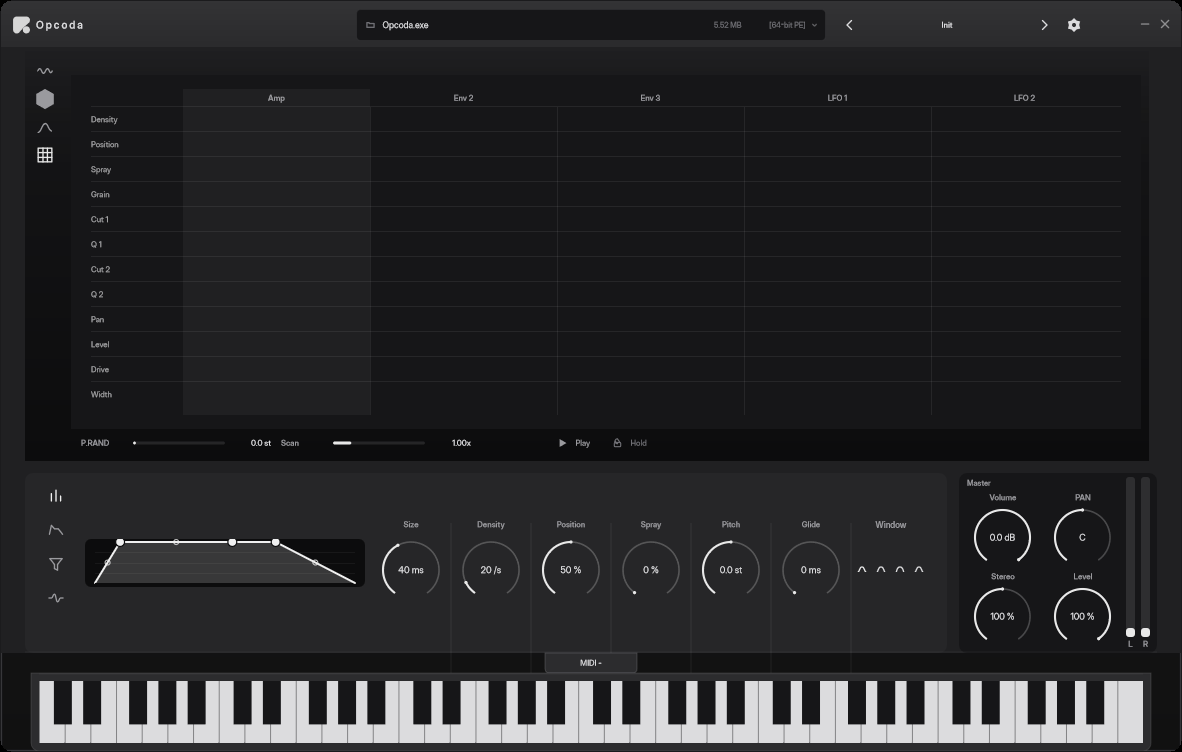
\includegraphics[width=\textwidth]{../assets/screenshots/opcoda-ui.png}
  \caption{The Opcoda interface: display and transport on top, the parameter
  panel and the master section below, and the MIDI keyboard drawer.}
  \label{fig:ui}
\end{figure}

\section{The Interface}
The window is divided in four areas:

\begin{itemize}
  \item \textbf{Header} --- preset name, the file field (path, size and format of
  the material) and the theme button.
  \item \textbf{Display} --- the waveform of the material with the transport
  controls (\textbf{Play}, \textbf{Hold}), the page buttons for the hex view,
  and four view buttons on the left edge: \textbf{WAVE}, \textbf{HEX},
  \textbf{ENTROPIA} and \textbf{MATRIX}.
  \item \textbf{Parameter panel} --- the four module tabs (Grain, Envelope,
  Filter, Mod) with their knobs, plus the master section on the right.
  \item \textbf{Keyboard drawer} --- the MIDI keyboard, opened and closed with
  the \texttt{MIDI - / MIDI +} tab under the chassis.
\end{itemize}

\subsection{The display views}
\begin{itemize}
  \item \textbf{WAVE} --- the waveform of the material with the region and the
  playhead.
  \item \textbf{HEX} --- the bytes of the file, with page navigation
  (Page Up/Page Down, Home/End).
  \item \textbf{ENTROPIA} --- the entropy curve of the material over its length.
  \item \textbf{MATRIX} --- the modulation matrix (see Section \ref{sec:matrix}).
\end{itemize}

\section{Parameters}

\subsection{Grain}
The grain section defines the cloud itself: how big each grain is, how many
per second, where they read from the file, and how they are tuned.

\paramtable{
\param{Size}{1 -- 2000 ms}{40 ms}{Grain length. Short grains (5--30 ms) give a fine, pointillist texture; long grains (100 ms+) smear the material into drones and pads. The scale is expanded around 100 ms, where most of the action happens.}
\param{Density}{1 -- 200 /s}{20}{Grains per second. Low densities isolate single grains (1--5 /s for rhythmic stutters); high densities fuse them into a continuous tone. Above ~50 /s the grain rate passes the audio rate and the texture becomes a tone.}
\param{Position}{0 -- 100 \%}{50 \%}{Read position in the file. With Play off, the grains read around this point; with Play on, the playhead advances and Position defines the offset. Automate it or modulate it for scrubbing and tape-style moves.}
\param{Spray}{0 -- 100 \%}{0 \%}{Random spread of the read position around Position. Small values humanize; large values scatter the grains across the whole file for clouds and clusters.}
\param{Pitch}{-48 -- +48 st}{0 st}{Transposition in semitones. Negative values slow down and darken (octave down = -12); positive values brighten. Quantized in semitones, with the exact tuning visible under the knob.}
\param{Glide}{0 -- 2 s}{0 s}{Glide time between notes. When you play legato, the pitch slides to the new note over this time instead of jumping.}
\param{Window}{4 shapes}{Hann}{Grain window shape. \textbf{Hann} is smooth and neutral; \textbf{Gaussian} is rounder and softer; \textbf{Hamming} has a flatter top (more click energy); \textbf{Blackman} is the smoothest and widest (fewer artifacts, softer attacks).}
}

\subsection{Envelope}
The envelope shapes every note: how the grain cloud fades in, sustains and
out. It is drawn as a single line in the display, with the four stages
always visible.

\paramtable{
\param{Attack}{1 -- 2000 ms}{5 ms}{Time to reach full level after the note-on. Short attacks click and punch; long attacks swell in slowly (pads, reverse-style textures).}
\param{Decay}{1 -- 2000 ms}{100 ms}{Time to fall from full level to the sustain level.}
\param{Sustain}{0 -- 100 \%}{100 \%}{Level held while the note is down.}
\param{Release}{1 -- 2000 ms}{50 ms}{Time to fade to silence after the note-off.}
\param{Attack Curve}{-100 -- +100 \%}{0 (LIN)}{Curvature of the attack ramp. Negative values make it fast-then-slow (exponential), positive slow-then-fast (logarithmic); 0 is linear.}
\param{Decay Curve}{-100 -- +100 \%}{0 (LIN)}{Curvature of the decay stage, same convention as the attack curve.}
\param{Release Curve}{-100 -- +100 \%}{0 (LIN)}{Curvature of the release stage, same convention.}
}

\subsection{Filters}
Two filters process the grain cloud, each with its own type, cutoff,
resonance and drive. The first filter also reacts to keytracking and to the
envelope; the second is static unless modulated from the matrix.

\paramtable{
\param{F1 Type}{4 types}{Low-pass}{Low-pass, High-pass, Band-pass or Notch. The buttons are on the left of each filter row.}
\param{F1 Cutoff}{20 Hz -- 20 kHz}{20 kHz}{Cutoff frequency (logarithmic scale, centred at 1 kHz). Fully open by default.}
\param{F1 Q}{0.5 -- 12}{0.71}{Resonance. 0.71 is Butterworth (flat); higher values add a peak at the cutoff (up to self-oscillating territory at the top of the range).}
\param{F1 Slope}{12 / 24 dB}{12 dB}{Slope steepness: 12 dB/oct (one pole) or 24 dB/oct (two poles).}
\param{F1 Drive}{0 -- 24 dB}{0 dB}{Gain into the first filter, for saturation and grit. Higher values compress and color the sound before the cutoff.}
\param{F1 Keytrack}{0 -- 100 \%}{0 \%}{How much the cutoff follows the played pitch (positive = higher notes open the filter). At 100 \% the filter tracks the keyboard fully.}
\param{F1 Env}{-100 -- +100 \%}{0 \%}{How much the envelope opens (positive) or closes (negative) the first filter. The classic envelope-to-cutoff amount.}
\param{F2 Type}{4 types}{Low-pass}{Low-pass, High-pass, Band-pass or Notch for the second filter.}
\param{F2 Cutoff}{20 Hz -- 20 kHz}{20 kHz}{Cutoff frequency of the second filter.}
\param{F2 Q}{0.5 -- 12}{0.71}{Resonance of the second filter.}
}

\subsection{Modulation (LFO)}
The LFO modulates one destination with a free-running or tempo-synced
wave. The wave is drawn as two scrolling cycles next to the controls: the dim
line is the full shape, the bright line is what the depth lets through.

\paramtable{
\param{Rate}{0 -- 20 Hz}{1.0 Hz}{LFO speed in free mode. At 0 the LFO stops; the sweet spots are 0.1--2 Hz for slow sweeps and 4--8 Hz for tremolo/roll effects.}
\param{Depth}{0 -- 100 \%}{0 \%}{How much the LFO moves the target. At 0 the target stays still (the waveform still scrolls, at full height, as a preview).}
\param{Target}{4 targets}{Pitch}{What the LFO modulates: Pitch, Density, Cutoff (first filter) or Position.}
\param{Wave}{5 shapes}{Sine}{Sine (smooth), Tri (linear ramps), Saw (ramp with a jump), Square (on/off) or S\&H (sample and hold, random per cycle).}
\param{Steps}{1 -- 16}{16}{Number of steps the wave is quantized to. 16 is smooth; low values (2--4) turn the LFO into a stepped sequencer. Only active when the wave is not a sine/triangle at 16.}
\param{Sync}{Free / Sync}{Free}{Free runs on the Rate knob; Sync locks the LFO to the host tempo and reveals the division control instead of the rate.}
\param{Div (sync)}{12 divisions}{1/4}{Musical division when synced: 1/1 up to 1/16T (including dotted and triplet forms). 1/4 at 120 BPM is 2 Hz.}
}

\subsection{Master}
The master section sits on the right of the panel: the output volume, the
stereo image and the per-grain level, with a vertical L/R meter below.

\paramtable{
\param{Volume}{-60 -- 0 dB}{0 dB}{Output volume. Below -60 dB the display shows $-\infty$. The meter shows the level in dBFS per channel, with the peak held.}
\param{Pan}{-100 -- +100}{Center}{Stereo position of the grain cloud. Center is 0; negative is left, positive is right.}
\param{Stereo Width}{0 -- 200 \%}{100 \%}{Width of the stereo image. 0 \% is mono; 100 \% is the natural width; up to 200 \% widens beyond the source (watch for phase in mono).}
\param{Grain Level}{0 -- 100 \%}{100 \%}{Level of the grain layer alone (before the master volume). Automate it for fades without touching the output.}
}

\subsection{Waveform View: Randomization and Scan}
Two sliders live in the display footer, next to the Play and Hold buttons:

\paramtable{
\param{P.RAND}{0 -- 12 st}{0 st}{Random detune applied per grain. 0 is off; 2--7 st gives a chorus/ensemble width; 12 st scatters the grains across an octave (chaos, bells).}
\param{Scan}{0.25 -- 4.00$\times$}{1.00$\times$}{Scan speed multiplier. 1.00$\times$ follows the file at real time; 0.25$\times$ slows the scan (4$\times$ longer file, darker motion); 4$\times$ scrubs forward fast.}
}

\subsection{Modulation Matrix}
\label{sec:matrix}
The matrix routes up to eight modulation sources to the parameters of the
voice. Open it with the \textbf{MATRIX} view button. Each row is a
destination; each column is a source; each cell is the amount of that route.

\begin{itemize}
  \item \textbf{Sources (columns)} --- \textbf{Amp} (velocity of the note),
  \textbf{Env} (the amplitude envelope), \textbf{LFO} (the LFO output),
  \textbf{Key} (keytracking, higher notes = more) and \textbf{Wheel} (the
  mod wheel, CC1).
  \item \textbf{Destinations (rows)} --- Pitch, Density, Position, Spray,
  Grain, Cut 1, Q 1, Cut 2, Q 2, Pan, Level, Drive and Width.
  \item \textbf{Amounts} --- each cell shows the amount as a percentage: drag
  up to add, down to subtract. Positive values push the parameter up, negative
  pull it down. Double-click or right-click clears the route. The bar at the
  base of the cell shows the magnitude.
\end{itemize}

A route writes directly into the parameter list (slots 1--8); it does not need
any other state. Eight routes exist; when they are full, reuse an existing
cell (change source or destination) instead of adding new ones.

\section{Playing Opcoda}
\subsection{Transport}
\begin{itemize}
  \item \textbf{Play} --- starts/stops the scan (space bar).
  \item \textbf{Hold} --- freezes the playhead where it is (H); press again to
  resume. While held, the grains keep playing around the frozen position.
  \item \textbf{Page buttons} (hex view) --- Page Up/Page Down, Home and End
  move through the file.
  \item \textbf{A} --- snaps the current selection to the nearest PE section
  (when a section list exists).
\end{itemize}

\subsection{Computer keyboard}
The virtual keyboard accepts the computer keys:
\texttt{A W S E D F T G Y H U J K} play a chromatic octave and a half
(C to C), with \texttt{K} also focusing the keyboard. The same notes can be
played with a MIDI controller.

\subsection{Presets}
The preset selector in the header (arrows + name) browses the factory
programs; the folder button opens the theme/audio settings. Presets capture
every parameter of the plugin, including the modulation matrix.

\section{Troubleshooting}
\begin{itemize}
  \item \textbf{The plugin does not appear in the DAW} --- rescan the VST3
  folder; Opcoda is at \texttt{Common Files\textbackslash VST3\textbackslash Opcoda.vst3}.
  Opcoda is an instrument: it needs a MIDI track with the plugin on it.
  \item \textbf{No sound} --- check the master Volume, the grain level and
  that a file is loaded; the envelope must be open (Attack/Release small).
  \item \textbf{The standalone opens with strange parameter values} --- delete
  \texttt{\%APPDATA\%\textbackslash Opcoda\textbackslash Opcoda.settings} to reset.
  \item \textbf{The keyboard drawer does not open} --- use the \texttt{MIDI +}
  tab under the chassis; the drawer slides out without resizing the window.
\end{itemize}

\clearpage
\appendix
\section{Parameter Reference}
The complete parameter list, alphabetically, with ranges and defaults. The
modulation matrix parameters \texttt{m1..m8} (src/dst/amt) are listed last.

\begingroup
\small
\begin{longtable}{@{}>{\raggedright\arraybackslash}p{24mm}>{\raggedright\arraybackslash}p{30mm}>{\raggedright\arraybackslash}p{14mm}>{\raggedright\arraybackslash}p{30mm}@{}}
\toprule
\textbf{ID} & \textbf{Name} & \textbf{Default} & \textbf{Range} \\
\midrule
\endfirsthead
\toprule
\textbf{ID} & \textbf{Name} & \textbf{Default} & \textbf{Range} \\
\midrule
\endhead
\bottomrule
\endfoot
grain & Grain Size & 40 ms & 1 -- 2000 ms \\
density & Density & 20 & 1 -- 200 /s \\
position & Position & 50 \% & 0 -- 100 \% \\
spray & Spray & 0 \% & 0 -- 100 \% \\
pitch & Pitch & 0 st & -48 -- +48 st \\
glide & Glide & 0 s & 0 -- 2 s \\
window & Window & Hann & Hann / Gaussian / Hamming / Blackman \\
volume & Volume & 0 dB & -60 -- 0 dB \\
pan & Pan & Center & -100 -- +100 \\
width & Stereo Width & 100 \% & 0 -- 200 \% \\
grainlevel & Grain Level & 100 \% & 0 -- 100 \% \\
pitchrand & Pitch Random & 0 st & 0 -- 12 st \\
scanspeed & Scan Speed & 1.00$\times$ & 0.25 -- 4.00$\times$ \\
attack & Attack & 5 ms & 1 -- 2000 ms \\
decay & Decay & 100 ms & 1 -- 2000 ms \\
sustain & Sustain & 100 \% & 0 -- 100 \% \\
release & Release & 50 ms & 1 -- 2000 ms \\
atkcurve & Attack Curve & 0 & -100 -- +100 \% \\
deccurve & Decay Curve & 0 & -100 -- +100 \% \\
relcurve & Release Curve & 0 & -100 -- +100 \% \\
f1type & Filter 1 Type & Low-pass & Low-pass / High-pass / Band-pass / Notch \\
f1cutoff & Filter 1 Cutoff & 20 kHz & 20 Hz -- 20 kHz (log) \\
f1q & Filter 1 Q & 0.71 & 0.5 -- 12 \\
f1slope & Filter 1 Slope & 12 dB & 12 / 24 dB \\
f1drive & Filter 1 Drive & 0 dB & 0 -- 24 dB \\
f1keytrack & Filter 1 Keytrack & 0 \% & 0 -- 100 \% \\
f1env & Filter 1 Env & 0 \% & -100 -- +100 \% \\
f2type & Filter 2 Type & Low-pass & Low-pass / High-pass / Band-pass / Notch \\
f2cutoff & Filter 2 Cutoff & 20 kHz & 20 Hz -- 20 kHz (log) \\
f2q & Filter 2 Q & 0.71 & 0.5 -- 12 \\
lforate & LFO Rate & 1.0 Hz & 0 -- 20 Hz \\
lfodepth & LFO Depth & 0 \% & 0 -- 100 \% \\
lfotarget & LFO Target & Pitch & Pitch / Density / Cutoff / Position \\
lfowave & LFO Wave & Sine & Sine / Tri / Saw / Square / S\&H \\
lfosync & LFO Sync & Free & Free / Sync \\
lfodiv & LFO Div & 1/4 & 12 divisions \\
lfosteps & LFO Steps & 16 & 1 -- 16 \\
m1..m8 src & Route Source & Off & Off / LFO / Env / Velocity / Key / Wheel / CC74 / CC71 / Entropy \\
m1..m8 dst & Route Destination & Off & 13 destinations \\
m1..m8 amt & Route Amount & 0 \% & -100 -- +100 \% \\
\end{longtable}
\endgroup

\vfill
\noindent{\color{mid}\sffamily\small bloodworm trax $\cdot$ Opcoda 0.1.0 $\cdot$ Manual version 1.0}

\end{document}